\subsection{a}
\lstinputlisting[caption={Topic 3. Question a. Note all code per topic belongs to same file }]{"./files/topic 3/a.m"}

\subsection{b}
\begin{figure}[h]
    \centering
    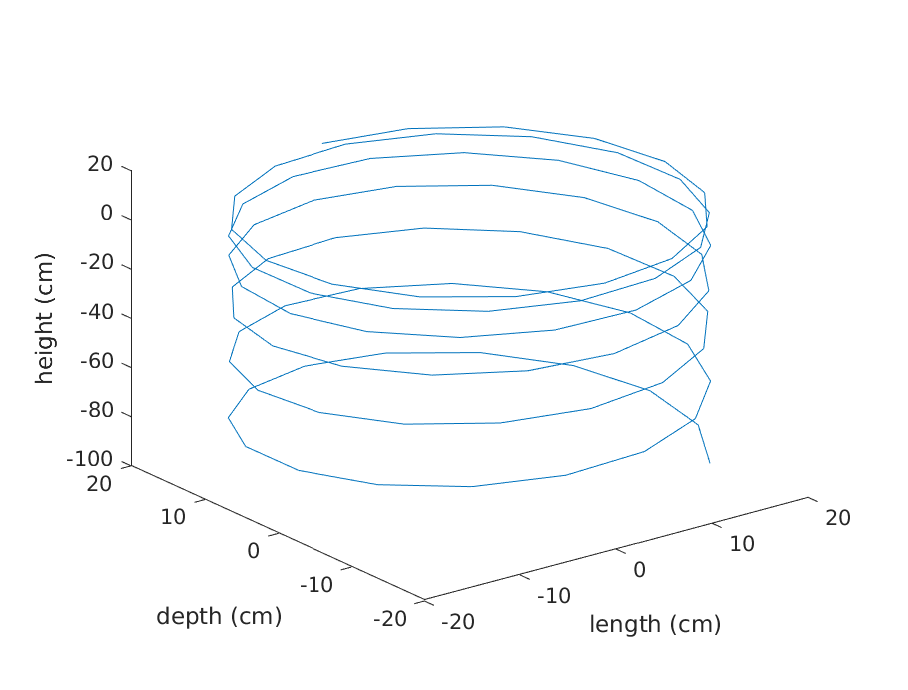
\includegraphics[scale=0.7, center]{./eps/topic3_b.eps}
    \caption{Particle position from $t=0$s to $t=40$s with 0.4 second intervals.}
    \label{fig:Topic3-b}
\end{figure}
\lstinputlisting[caption={Code for Topic 3. Question b. Note all code per topic belongs to same file}]{"./files/topic 3/b.m"}

\subsection{c}
Given that the speed is the modulus of velocity,
\begin{equation}
        \left| \overrightarrow{v}(15) \right| = \left| \begin{bmatrix}
            20\cos(15)\\ -20\sin(15) \\ -\frac{2}{16}15
        \end{bmatrix} \right|
        =
        \left| \begin{bmatrix}
        -15.1938 \\ -13.0058 \\ -1.8750
        \end{bmatrix} \right|
        =
        20.0877 \text{ cms$^{-1}$ }
\end{equation}

\subsection{d}
\begin{figure}[h]
    \centering
    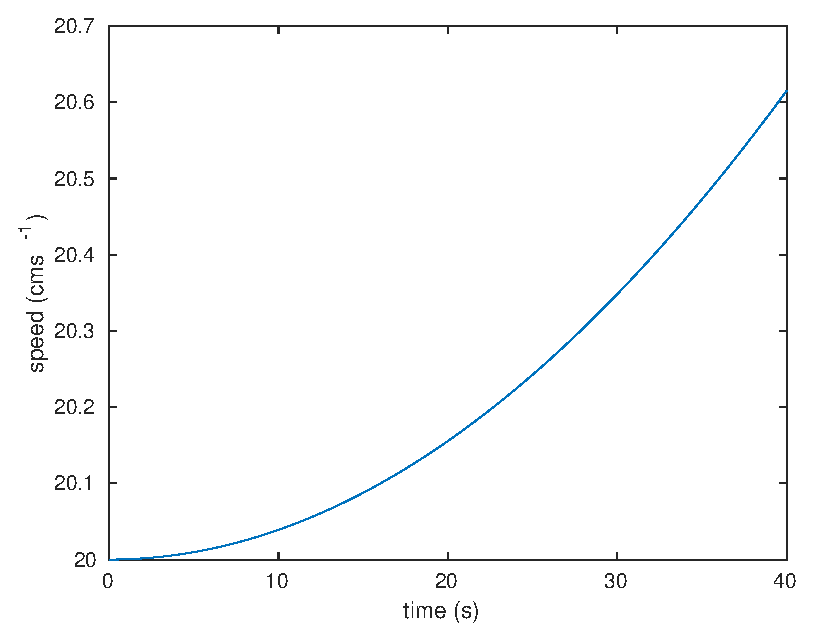
\includegraphics[scale=0.7, center]{./eps/topic3_d.eps}
    \caption{Particle speed varying with time.}
    \label{fig:Topic3-d}
\end{figure}

\lstinputlisting[caption={Topic 3. Question d. Note all code per topic belongs to same file}]{"./files/topic 3/d.m"}